\section{Org chart orientation
\label{org-chart-orientation}}
A common method of describing relations within the bureaucracy is the organization chart (colloquially, the "org chart"). Normally the CEO is at the top of the chart, middle management is in the middle, and managed employees are at the bottom. 

There are emotional connotations to alternative layouts
\begin{itemize}
\item CEO at the bottom
\item CEO on the left
\item CEO on the right
\item CEO as the center of a star
\end{itemize}


\begin{figure}
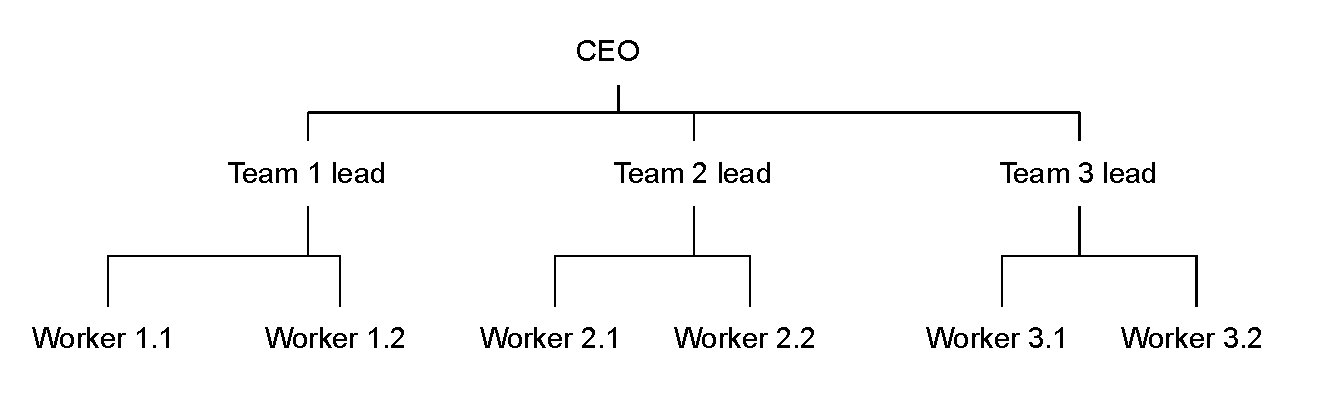
\includegraphics[width=0.8\textwidth]{images/org-chart-orientation-ceo-at-top.pdf}
\caption{Standard orientation. Role with most responsibility is at top. Left-right ordering is irrelevant in this view.}
\end{figure}

\begin{figure}
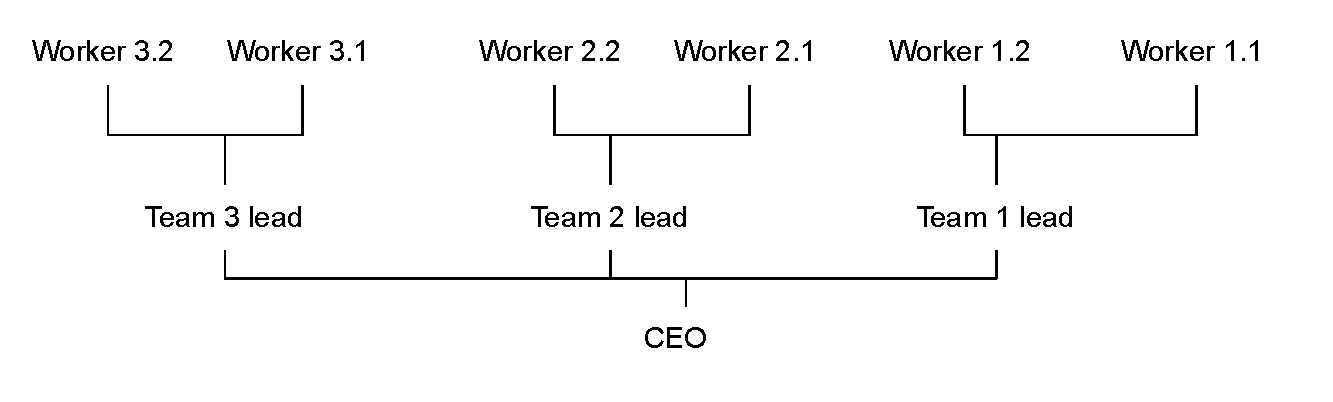
\includegraphics[width=0.8\textwidth]{images/org-chart-orientation-ceo-at-bottom.pdf}
\caption{Flipping the orientation presents a more realistic burden}
\end{figure}

\begin{figure}
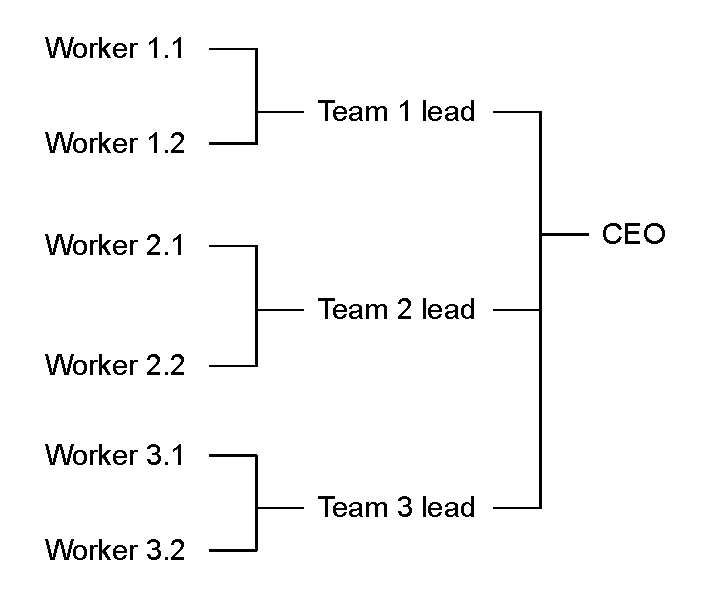
\includegraphics[width=0.8\textwidth]{images/org-chart-orientation-ceo-leads.pdf}
\caption{I'm used to time flowing from left to right, so the CEO leads the charge}
\end{figure}

\begin{figure}
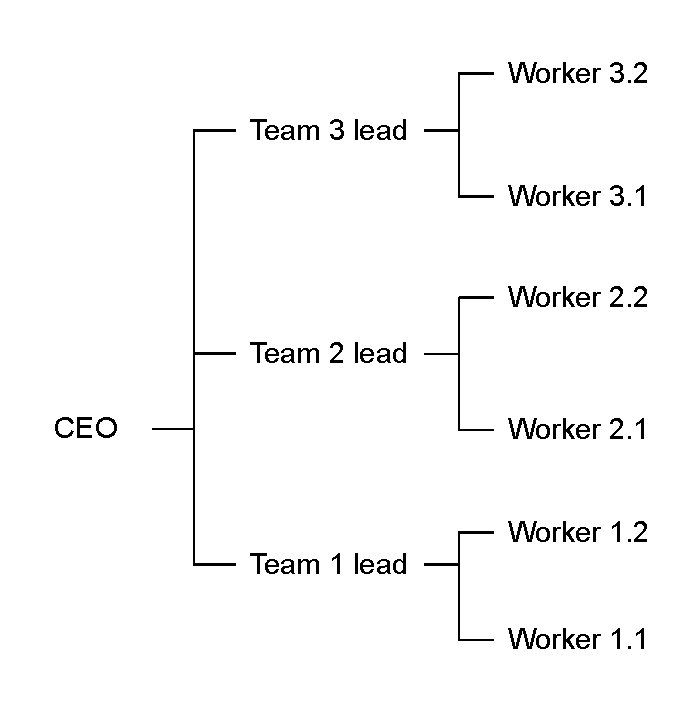
\includegraphics[width=0.8\textwidth]{images/org-chart-orientation-workers-lead.pdf}
\caption{My favorite: ``chariot view''.}
\end{figure}
